\documentclass[a4paper]{article}

\usepackage[english]{babel}
\usepackage[utf8]{inputenc}
\usepackage{amsmath}
\usepackage{amssymb}
\usepackage{graphicx}
\usepackage[colorinlistoftodos]{todonotes}
\usepackage[margin=1in]{geometry}
\usepackage{graphicx}

\setlength\parindent{0pt}

\newcommand{\ledd}{L_{\mathrm{Edd}}}
\newcommand{\medd}{\dot{M}_{\mathrm{Edd}}}
\newcommand{\Comment}[2]{ [{\color{red}\sc #1 :} {{\color{cyan} \it #2}}]}
\newcommand{\gcm}{g/$\mathrm{cm}^3$}

\title{Ay125 Final Review Questions}

\author{Anna Ho}

\date{\today}

\begin{document}
\maketitle

\begin{enumerate}

\item \textbf{Calculate from first principles the density at which degenerate electrons become relativistic. What temperature would be required to lift the degeneracy?} \\

\textcolor{blue}{Additions by Bhawna in blue.}

Degenerate electrons become relativistic when 

\begin{equation}
p_F c = m_e c^2
\end{equation}

and for a degenerate Fermi gas, we can write the following relation between electron density and Fermi momentum:

\begin{equation}
n_e = \frac{8 \pi}{3} \left( \frac{p_F}{h} \right)^3
\end{equation}

Solving for $n_e$, we have

\begin{equation}
n_e = \frac{8 \pi}{3} \left( \frac{m_e c}{h} \right)^3
\end{equation}

The condition for degeneracy is $kT \ll \epsilon_F$, so to lift the degeneracy you would need $kT = \epsilon_F$. 

\begin{equation}
T = \frac{\epsilon_F}{k} = \frac{1}{k} \left( \sqrt{m_e^2 c^4 + p_F^2 c^2} - m_e c^2 \right)
\end{equation}

We should probably also know the various limits of this equation. \newline

\item \textbf{Derive the mass-radius scaling for low mass white-dwarfs (Fermi energy less than $m_e c^2$) and high mass white-dwarfs (Fermi energy more than $m_e c^2$), and explain the origin of the Chandrasekhar mass limit.} \newline

We can derive an approximate scaling for the \textbf{mass-radius relationship} in the non-relativistic limit, starting with the equation of hydrostatic equilibrium and the equation of state for a non-relativistic degenerate electron gas.

$$ \frac{dP}{dr} = -\frac{GM}{R^2} \rho \propto \frac{G M^2}{R^5} $$

So,

$$ P \propto \frac{G M^2}{R^4} $$

And the equation of state is:

$$ P \sim \frac{\hslash^2}{m_e} n_e^{5/3} $$

Putting these two together, we get

$$ R \sim \frac{\hslash}{m_e} \frac{1}{G m_b^{5/3}} M^{-1/3} $$

For a high mass WD with relativistic electrons \textcolor{blue}{(the degeneracy pressure forces electrons to reach energies highly exceeding their rest mass energies)}, the equation of state is, instead, 

$$ P \propto n_e^{4/3} $$

As a result, $R$ is not dependent on $M$ at all. In fact, $M$ simply takes on one value: the fundamental mass limit called the \textbf{Chandrasekhar limit}, $M_{Ch}$. Qualitatively, here's how you can understand the origin of this limit: as you crank up the central density so that $\rho_c \rightarrow \infty$, the electrons become more and more relativistic throughout the star, and the mass asymptotically approaches the value $M_{ch}$ as $R \rightarrow 0$. This mass limit represents the maximum possible mass of a white dwarf, and its dependence on composition is contained entirely in $\mu_e$ for a cold, perfect gas. 

\begin{equation}
M \rightarrow 1.457 \left( \frac{2}{\mu_e} \right)^2 M_\odot 
\end{equation}

\item \textbf{Derive the Chandrasekhar mass limit by considering the energy of a relativistic gas particle}

The Fermi energy of a relativistic gas particle in a degenerate gas is

$$ E_F \sim p_F c $$

And the Fermi momentum is always

$$ p_F \sim \hslash n_e^{1/3} $$

So, 

$$ E_F \propto \hslash n^{1/3} c \propto \frac{\hslash c N^{1/3}}{R} $$

Each fermion has a gravitational energy

$$ E_G \propto - \frac{G M m_B}{R} = \frac{G N\textcolor{blue}{_B} m_B^2}{R} $$

\textcolor{blue}{where $m_B$ and $N_B$ are mass of a single baryon and total number of baryons, respectively. Also, $N_B$ $\sim$ 2$N$}

So, the total energy is 

$$ E = \frac{\hslash c N^{1/3}}{R} - \frac{\textcolor{blue}{2}G N m_B^2}{R} $$

If $N$ is very large, $ E < 0 $, and you can make $E$ more and more negative by decreasing $R$, so there's no stable equilibrium. So, to achieve equilibrium you just set $ E = 0 $. Thus,

$$ N_{max} \propto \left( \frac{\hslash c}{\textcolor{blue}{2}G m_B^2} \right)^{3/2} $$

This gives,

$$ M_{\mathrm{max}} \propto N_{\mathrm{max}} \, m_B \propto 1.5 M_\odot $$

\item \textbf{What actually sets the maximum mass of a white dwarf, and how does this depend on composition?}

In HW1, we mentioned that the maximum mass can be set by the pycnonuclear reactions which can fuse WDs in $\ll 10^5 $ yr when the central densities are higher than $10^6, 10^9,$ and $10^{10} \ \rm g \ cm^{-3}$ for H, He, and C WDs respectively. Pycnonuclear reactions are nuclear fusions that happen to nuclei confined in lattice structures at high density \textcolor{blue}{and very low temperatures ($T \sim 0 K$). Unlike thermonuclear reactions, the rates of these reactions are not sensitive to temperature, but grow exponentially with increasing densities. The threshold densities for such reactions to happen is, as we saw, different for different WD compositions}.

\item \textbf{Outline the principles of calculating white dwarf cooling, and the relation between luminosity, age and mass of white dwarfs.}

You can think of a WD like a degenerate isothermal metal ball, with heat carried by electron conduction \textcolor{blue}{(this is because the opacities for radiative transport are low in lack of vacant energy levels for electrons to jump to by absorption of photons)}, with a non-degenerate blanket that has a temperature gradient. This ``blanket'' is basically nondegenerate surface layers that are in ``radiative equilibrium'': matter is in local thermodynamic equilibrium with an energy flux carried outward by photon diffusion (heat transport by radiation). 

Let's begin with the Eulerian form of the temperature equation of stellar structure, which you can define by considering radiative transport as a diffusion process. 

\begin{equation}
\frac{dT}{dr} = \frac{-3 \, \kappa \, \rho \, L}{16 \, \pi \, a \, c \, T^3 \, r^2}
\end{equation}

Approximate the opacity using Kramer's opacity, which arises from photoionization of atoms (``bound-free" transitions) and inverse Bremsstrahlung of free electrons (``free-free" transitions):

\begin{equation}
\kappa = \kappa_0 \rho T^{-3.5}
\end{equation}

Now, divide the equation of hydrostatic equilibrium by the temperature equation of stellar structure and get

$$ \frac{dP}{dT} = \frac{4ac}{3} \frac{4 \pi G M}{\kappa_0 L} \frac{T^{6.5}}{\rho} $$

Use the equation of state of an ideal gas to replace $\rho$:

\begin{equation}
P = \frac{\rho}{\mu m_u} kT
\end{equation}

And integrate the resulting differential equation using the condition that $P = 0$ when $T = 0$:

$$ P dP = \frac{4ac}{3} \frac{4 \pi G M}{\kappa_0 L} \frac{k}{\mu m_u} T^{7.5} dT $$

\noindent Replacing $P$ with $\rho$ from the equation of state gives

$$ \rho \propto M^{1/2} \, L^{-1/2} \, T^{3.25} $$

The problem with this is that it breaks down when the electrons become degenerate. This occurs when the nondegenerate expression for electron pressure becomes the degenerate expression:

$$ \rho T \propto \rho^{5/3} $$

Or,

$$ \rho \propto T^{3/2} $$

Plugging this in:

$$ L \propto M \, T^{3.5} $$

So, now we have a relationship between luminosity, mass, and temperature! Let's turn to cooling.

The \textbf{cooling rate} is the rate of change of the thermal energy $U$ of the white dwarf:

\begin{equation}
U = \frac{3}{2} kT \frac{M}{A \, m_u}
\end{equation}

Let the cooling rate $-dU/dt$ equal to the luminosity. Then you get,

$$ -\frac{d}{dt} \left( \frac{3kT/2}{A m_u} \right) = CT^{7/2}$$

Integrate to get an expression for time, taking the limit that the initial temperature is way larger than the final temperature:

$$ t_{\mathrm{cool}} \propto \frac{TM}{L} $$

And plugging in our expression for luminosity,

$$ t_{\mathrm{cool}} \propto \left( \frac{L}{M} \right)^{-5/7}$$

\item \textbf{Discuss what sets the lower end of the white dwarf luminosity function. Does it depend on mass? Is crystallization expected, and how does it affect cooling?}

Basically, they're created very hot, and then they cool down. The lower limit on temperature is set by a couple of things:

\begin{enumerate}
\item Age: they can't cool down for longer than the age of the universe
\item If it's a massive WD, it gets colder at the center until the ions crystallize, so the temperature plummets and they fade rapidly because there's hardly any heat left at the center. 
\end{enumerate}

You can use these white dwarf cooling sequences to age-date globular clusters. 

We have neglected one important effect in particular: crystallization of the ion lattice. At low temperatures (and low luminosity) the lattice vibrations of the ions are more important than the free thermal motion. So, you get more rapid cooling. 
In a white dwarf, the electrons have most of the energy, but most of the heat is in the ions. 
If you crank up the density, the ions become degenerate and you get a neutron star. If you crank up the temperature, you get crystallization, which means that the heat content drops. The temperature at which this happens increases steeply with mass.

\textcolor{blue}{Writing my impression of the answer:\\ The low luminosity end of the WD luminosity function has a steep drop governed by the time that has passed since the WD started cooling. The longest that the WDs could have been cooling would be the age of the galaxy in which they are, or more liberally, the age of the universe at the most. Since a more massive WD has smaller radius (hence lower surface area) than its less massive counterpart of the same age, it cools down slower and would exhibit a higher luminosity than the latter.\\
As the temperature drops, the thermal kinetic energy of heavy element ions such as C and O present in the interiors of WDs drops enough that they can now crystallize into lattice structures maintained by Couloumb repulsion. By the virtue of additional luminosity from the release of crystal latent heat, this process effectively slows down the cooling rate until the WD fully crystallizes.}

\item \textbf{Discuss the atmospheric composition of white dwarfs, and the physical reasons for these.}

White dwarfs are classified into two distinct families according to the main constituent of their surface. 85\% of white dwarfs are \textbf{DA white dwarfs}: the surface composition consists almost entirely of H with at most traces of other elements. The remaining 15\% or so are \textbf{non-DA white dwarfs}: they are H-deficient with He-rich atmospheres. They are thought to be H-deficient because their progenitor underwent some kind of violent episode, like a thermal flash or a \textcolor{blue}{recent} merger. The ratio of non-DA/DA WDs decreases with a decrease in surface temperature due to the gravitational setting of heavy elements, which generally takes place quite fast. They can be broken further into subclasses: DO have singly ionized He, DB have strong neutral He lines \textcolor{blue}{(with lower $T_\mathrm{eff}$ than DOs to facilitate recombination of He$^{+}$)}, and DC, DQ, and DZ have \textcolor{blue}{featureless continuum spectra,} carbon \textcolor{blue}{lines (due to convective mixing)} and metal \textcolor{blue}{lines (due to accretion) respectively}. There's also a new type, called \textbf{hot DQ white dwarfs} that have carbon-dominated atmospheres. They are thought to be the result of convective mixing.

\item \textbf{What are novae? What determines whether or not there is a thermonuclear runaway near the surface of an accreting white dwarf? Is the burning a detonation (explosive burning behind
a shock front)?}

For the price of one calculation, you can do novae (white dwarf accretors), x-ray bursts (neutron star accretors), shell flashes...

Suppose the compact object is accreting at the Eddington Luminosity. You can estimate the energy released by

$$ \ledd = 4 \pi R^2 \sigma T^4 $$

For a white dwarf, you get $kT \sim 100\,\mathrm{eV}$ and for a neutron star you get $2\,\mathrm{keV}$ which is right smack in the x-ray band.

Imagine that you're dropping hydrogen on. There's a shock at the surface layer. It becomes hotter and denser as you accrete more stuff, until nuclear fusion sets in. In order to reach a steady state, you have to have some radiation flux coming out from the cooling of the white dwarf (such that flux out the top is equal to the flux out the bottom). You can think of the pressure at the bottom as $g \Sigma$ (the column density). The column density changes with accretion:

$$ \dot{\Sigma}_\mathrm{acc} = \frac{\dot{M}}{4 \pi R^2} $$

As you accrete, hydrogen is fusing into heavier particles, so with time the pressure decreases because there are simply fewer and fewer particles.

Now, how does pressure scale with accretion rate? 
In the low $\dot{M}$ limit, pressure increases as you increase the accretion rate. In the high $\dot{M}$ limit, the accretion material is very fluffy; you can build an infinite radiation-dominated star. 
At intermediate values, the pressure decreases as you increase the accretion rate. 
The shortest timescale I can undergo burning is hundreds of seconds, since these are the $\beta$ decay waiting times. 

For a neutron star and white dwarf, the stuff hydrostatically expands, it's not some instantaneous explosion. It's not in radiative equilibrium but it is in hydrostatic equilibrium because it's much slower than the pressure waves. The envelope becomes gravitationally unbound. 

They're not explosions: they're rapidly burning and expanding shells.

After three years or so, the nebula expanding shell becomes transparent and you can start to see the hot white dwarf, and it ionizes the nebula around it. 

You can get \emph{recurrent novae}: very massive, very high accretion rate systems. The time between flashes is on the order of $ t \sim \frac{\Delta M}{\dot{M}} $

\textcolor{blue}{Again, I'll just write my short version here:\\ Novae are manifestations of runaway fusion reactions triggered by the heat of accretion onto the WD from a companion. This phenomenon, also known as `unstable burning', leads to liberation of huge amounts of energy that violently blows away material from the white dwarf's surface and produces an extremely bright burst of light that we call Nova. From what I understand, whether or not thermonuclear runaway would happen is determined by the accretion rate. If the accretion rate is fast enough that the material (mostly H) keeps burning as it accretes on to the WD surface, there would be no unstable burning. So for unstable burning to happen, the accretion rates have to be slow such that the material can pile up on the WD surface without reaching burning temperatures and then burns all at once at a later time. The resulting energy from unstable nuclear burning in this case does not propagate through a shock front, but as a ``flame'' or a deflagration front instead.}

\item \textbf{Explain the phenomenon of accretion-induced collapse of a white dwarf, and the role played by electron capture. What other phenomena might prevent accretion-induced collapse?}

The white dwarf has a carbon-burning shell that's adding mass to the (O, Ne, Mg) core. As you gradually add mass, the following could happen:

\begin{enumerate}
\item (O, Ne, Mg) can undergo electron capture and fuse to form heavier things
\item Eventually becomes unstable and collapses
\item Competition between electron capture, transition to instability. Explosion? Partial explosion (only enough energy to unbind outer layers)? Collapses into a neutron star? An \emph{electron-capture supernova}? Accretion-induced collapse? (The former is a popular theory for how to produce a neutron star with a low kick velocity, and the latter is a popular theory for how to make a young neutron star in a globular cluster). 
\end{enumerate}

\textcolor{blue}{Heavier elements like magnesium and neon in an ONeMg WD are less susceptible to runaway fusion than carbon and oxygen, and are more likely to undergo the neutronization reactions that remove the electron degeneracy pressure support and causes the star to collapse. Therefore, if the accretion rates are small, an ONeMg WD will continue to gain mass till it reaches the Chandrashekhar limit and then collapse.\\ The role of electron capture reactions in this process is in the removal of electrons, and hence in the reduction of degeneracy pressure support.\\ For starters, runaway fusion of heavy elements before pressure support is taken away can stall the collapse. Speculation - Perhaps also high speed rotation, and heating from neutrinos?}

\item \textbf{Derive degeneracy pressure of free-neutrons and the free neutron analog of the white-dwarf mass-radius relation. How does, or does not, this calculation accurately represent the properties of neutron stars?}

(KT: Not very certain)
The derivation of the neutron degeneracy pressure and the mass-radius relation for neutron stars should be exactly the same as the free relativistic electron derivation for WDs \textit{if} neutrons are actually free. The trouble is that the unbound neutrons (as in, not in nuclei) are \textit{strong}ly interacting. Therefore, the free-fermion assumption we used in the WD derivation failed miserably. The actual mass-radius relation is still uncertain due to the fact that we (physicists, that is) don't know the equation of states at such densities very well.  

\item \textbf{Explain how one derives the most stable (minimum energy) nucleus as a function of density, including beta-capture/beta-decay, and the effects on the nuclei of free electrons, neutrons
and protons. In what circumstances are the minimum energy nuclei the ones that will actually be present in neutron stars?}

(KT) This is on page 42 in http://www.its.caltech.edu/$\sim$esp/ay125/BHWDNS-16-105.pdf

Normally, the most stable nucleus is the one with the maximum binding energy per nucleon. However, at higher densities, the Fermi energy is such that it is more energetically favorable for electrons to get captured into the nuclei ($\beta$-capture), raising the neutron number of the most stable nucleus. The energy density of a mixure of nuclei, free electrons, and free neutrons is given by 

$$ \epsilon = n_N M(A,Z) + \epsilon_e(n_e) + \epsilon_n(n_n) $$

where $\epsilon_i$ are the energy density of the free gas of electrons/neutrons. $M(A,Z)$ is the energy per nucleus, given by the \textit{semiempirical} mass formula, which you get from talking to a partical physicist. The most stable nucleus is given by $A$ and $Z$ that minimize $\epsilon$ as a function of $n_e$ and $n_n$. 

\item \textbf{Describe the structure of neutron stars from the core to the surface.}

The last km or so is where all the action happens. Let's break it down by layers.

\begin{description}

\item[Surface, $\rho < 10^6$ \gcm]. Temperatures and magnetic fields can significantly affect the equation of state. Above 10 meters, below 50 \gcm, you have mostly ionized atomic shells. Density rises by many orders of magnitude, your shells become pressure-ionized, all degenerate. At 10 meters, you have non-relativistic electrons below a density of around $10^6$, but once you get above that you have relativistic electrons.

\item[Outer crust, $10^6 < \rho < 10^{11}$] A solid region in which a Coulomb lattice of heavy nuclei coexists in $\beta$-equilibrium with a relativistic degenerate electron gas. At 200 meters (around $10^{10}$) you start to get neutronization. 

\item[Inner crust, $10^{11} < \rho < 10^{14}$] Lattice of neutron-rich nuclei together with a superfluid neutron gas and an electron gas. At 1 km, you start to get neutron drip at density $10^{11}$. When the energies are higher than the binding energy of neutrons, the neutrons are just as happy outside the nuclei as inside - so they begin dripping out. 

\item[Neutron liquid, $\rho > 10^{14}$] Superfluid neutrons with a smaller concentration of superfluid protons and normal electrons. You reach nuclear density at $10^{14}$. Above that, you're above nuclear density and have nuclear pasta, and ``all hell breaks loose.'' At these ridiculous high densities, atoms are no longer spherical; they arrange themselves into long chains to adjust the packing efficiency (reach a lower energy state). In the inner regions of neutron stars, neutrons are believed to pair and become superfluid. The electrons and protons become a superconductor. All neutron stars above a certain age are predicted to be superconducting at the center. 

\item[Core] I don't think anybody really knows! Quark matter? 

\end{description}




\item \textbf{Derive the vacuum dipole spin-down relation giving the rate of spin down of a pulsar with given spin frequency, moment of inertia magnetic dipole polar field or magnetic moment, and inclination angle. Explain what aspects of this calculation are believed to apply to real
pulsars.}

If the magnetic dipole is inclined by some angle $\alpha > 0$ from the rotation axis, it emits low-frequency electromagnetic radiation. The power of the magnetic dipole radiation from an inclined magnetic dipole is analogous to the Larmor formula for radiation from a rotating electric dipole:

$$ {P_{\rm rad} = {2 \over 3} { (
\ddot{m}_\bot )^2 \over c^3}}\rlap{\quad \rm } $$

For a uniformly magnetized sphere with radius $R$ and surface magnetic field strength $B$, the magnetic dipole moment is

$$ m = B R^3 $$

Letting $m =m_0 \exp ( - i \Omega t)$, you get

$$ P_{\rm rad} = {2 \over 3} { m_\bot^2 \Omega^4 \over c^3} = {2
m_\bot^2 \over 3 c^3} \biggl( {2 \pi \over P} \biggr)^4 = {2 \over 3
c^3} ( B R^3 \sin \alpha)^2 \biggl( {2 \pi \over P} \biggr)^4~ $$

And rotation energy is related to the moment of inertia by

$$ E_{\rm rot} = \frac{1}{2}I \Omega^2 = {2 \pi^2 I
\over P^2} $$. 

The moment of inertia is

$$ I = \frac{2}{5} M R^2 $$

To get the minimum magnetic field strength,

$$ P_{\rm rad} = - {d E_{\rm rot} \over d t} $$

$$ {2 \over 3 c^3} (B R^3 \sin \alpha)^2 \biggl( { 4 \pi^2 \over P^2}
\biggr)^2 = {4 \pi^2 I \dot{P} \over P^3} $$

$$ B^2 = { 3 c^3 I P \dot{P} \over 2 \cdot 4 \pi^2 R^6 \sin^2\alpha } $$

$$ B > \biggl( { 3 c^3 I \over 8 \pi^2 R^6} \biggr)^{1/2} (P \dot{P})^{1/2} $$

$$ \biggl( { B \over {\rm Gauss}}
\biggr) > 3.2 \times 10^{19} \biggl( 
{ P \dot{P} \over {\rm s} } 
\biggr)^{1/2} $$

(KT) The applicability of the vacuum dipole radiation might be limited by the following. 
(i) The frequency at which it radiates ($\sim$ the rotational frequency of about 1 Hz) is way below the plasma frequency of the ISM. Hence, that rediation cannot propagate. This luminosity ($\sim 10^5 \ L_{\odot}$ for Crab) is much larger than the radio luminosity observed from a pulsar, so it must be absorbed and reemitted from the ISM. 
(ii) The vicinity of a pulsar is unlikely vacuum. In the co-rotating frame, the electric field parallel to the surface need not be zero, and that produces a charge distribution outside. 

\item \textbf{Estimate the minimum rotation period of a neutron star. How does this compare to the
actual shortest measured pulsar period?}

This is set by the requirement that the centrifugal acceleration at the equator not exceed the gravitational acceleration.

$$ \Omega^2 R < {\frac{G M} {R^2}} $$

$$ {\frac{4 \pi^2 R^3} {P^2}} < GM $$

$$ P^2 > \biggl( { \frac{4 \pi R^3}{3}} \biggr) {\frac{3 \pi}{GM}} $$

Taking $ R = 10\,$km and $M = 1.4 M_\odot$, this is around 46 microseconds. The fastest known pulsar has $P = 1.4 \times 10^{-3}\,$seconds.

In fact, a rapidly spinning star becomes oblate, which increases the centrifugal acceleration and decreases the gravitational acceleration at the equator.

\item \textbf{At what photon wavelengths or energies have pulses been detected from pulsars, and what does each of them tell us about the location and nature of the emission? Is most of the rotational energy lost going into photons?}

There seems to be a picture where the radio emission originates from close to the stellar surface, while the high-energy emission may tend to be created further out. One would not expect an alignment of radio and high-energy profiles, as is typically observed. When alignment is observed (e.g. Crab pulsar) perhaps the observed radio emission is of different origin and more related to that at high energies. 

\begin{description}

\item[IR, Optical, UV] Pulsars are generally very weak optical sources. Optical pulses only detected in a few pulsars. Young and old pulsars have power law spectra, middle aged also have black body component produced by thermal emission from the polar cap or the whole surface. Crab pulsar's optical pulse profile is very similar to the x-ray and gamma ray one, suggesting that it's created by the same non-thermal radiation process, presumably at the same location. Mixture of thermal and non-thermal emission. 

\item[X-ray] 15 pulsars so far. More direct insight into the magnetospheric process than radio, because there are fewer complications in understanding it (e.g. propagation effects). In most cases you can do power law and/or black body fits to spectra. Similarities of x-ray profiles with radio pulse shapes suggest non-thermal magnetospheric origin of emission. There's one pulsar where the data can be described by a combination of a power law and two thermal blackbody components, possibly originating from two surface regions of different temperature. Mixture of thermal and non-thermal emission. 

\item[Gamma-ray] Highly pulsed, beamed and of non-thermal origin. Profiles typically double-peaked. 

\end{description}

\item \textbf{Describe the various observational manifestations of neutron stars and their sources of energy}

\begin{enumerate}

\item Accretion energy: Accretion-powered neutron stars: we're pretty sure we have a complete sample of those that are bright most of the time. 
\begin{description}
\item[LMXB] Accreting from Roche lobe overflow (orbital period 2-10 hours), many in the bulge.
\item[IMXB] Very short lifetimes
\item[HMXB] Accreting from a massive, O or B star wind (orbital period months)
\item[UCXB] WD and NS, orbital period minutes
\end{description}

\item Rotation energy: Rotation powered neutron stars

\begin{description}
\item[Radio pulsars] Currently around 2500, of which 250 are MSPs. 
\item[RRATs: Rotating RAdio Transients] 
\item[Gamma Ray Pulsars] Very high energy per particle, we only see these if they're bright in the gamma ray. Around 200 of them. 
\end{description}

\item Thermal energy: Cooling-powered neutron stars

\begin{description}
\item[XDINS: X-ray Dim Isolated Neutron Stars] If you're looking for cool things that are nearby, this is a great way to go. They undergo pulsations because they do have a magnetic field, with most of their heat coming out of the x-ray poles.  
\item[Compact Central Objects] There are 8 of these and they're in supernova remnants. 
\end{description}

\item Magnetic energy: Magnetic decay powered neutron stars

\begin{description}
\item[Magnetars] If you're isolated and rotating slowly, your only hope is your magnetic field. There are around 26 of these known. Anomalous x-ray pulsars, soft gamma-ray repeaters. They sufficiently ionize the Earth's atmosphere enough to affect radio transmission. These systems have magnetic fields of $10^{14}-10^{15}\,$G.
\end{description}

\end{enumerate}

\item \textbf{Describe how millisecond pulsars are formed.}

Millisecond pulsars are recycled: spun up by accreting mass and angular momentum from their companions, to the point that they emit radio pulses despite their relatively low magnetic field strengths $B \sim 10^8$ Gauss. Some are isolated, they were probably recycled via the standard scenario in binary systems, but the energetic MSPs eventually ablated their companions away. 

\item \textbf{What are magnetars and what provides their radiated energy?}

Magnetars are magnetic decay powered neutron stars. 
If you're isolated and rotating slowly, your only hope is your magnetic field. There are around 26 of these known. Anomalous x-ray pulsars, soft gamma-ray repeaters (although it's possible that eventually all of these will appear in the latter category). They sufficiently ionize the Earth's atmosphere enough to affect radio transmission. These systems have periods from 1-15 seconds and magnetic fields of $10^{14}-10^{15}\,$G. Most are found very close to massive star clusters. 
Radiation powered by magnetic field decay.

(KT) Magnetars that are born with short period (ms) are thought to be a central engine to long-period GRBs and some superluminous supernovae. In these cases, the radiated energy comes from the massive spin-down power due to a large magnetic torque. This mode of radiation doesn't last very long. 

\item \textbf{Derive, approximately or exactly up to dimensionless factors, the Bondi accretion rate onto a mass $M$ at rest in a homogeneous medium of density $\rho$ and speed of sound $c_s$. Explain the significance of the Bondi radius.}

Bondi accretion is the spherical accretion of interacting particles. We're in the non-relativistic, steady state limit. 

Begin with the Bernoulli Equation:

\begin{equation}
\frac{1}{2} u^2 + \int \frac{dP}{\rho} - \frac{GM}{r} = e = \mathrm{constant}
\end{equation}

Far away from the black hole, you can neglect the velocity $u$ because it goes as $\frac{1}{r^4}$. Out there, the conserved quantity is just the second two terms. You can write the first in terms of the sound speed:

$$ \int \frac{dP}{\rho} = \frac{1}{\gamma-1} c_s^2 $$

since $c_s^2 = \frac{\gamma P}{\rho}$. 

Thus, we have the conservation statement

$$ \frac{1}{\gamma-1} c_s^2 - \frac{GM}{r} = \frac{1}{\gamma-1} c_{s,\infty}^2 $$

The Bondi radius is where the sound speed has changed by order unity from its original value. It defines the radius of influence of the black hole. And, it marks the transition from subsonic (far from the BH) to supersonic (close to the BH). 

At supersonic speeds, 

\begin{equation}
r_\mathrm{Bondi} = \frac{GM}{c^2_\infty}
\end{equation}

At this transition point, the mass accretion rate is governed by conservation of mass:

$$ \dot{M} = 4 \pi r^2 \rho u = 4 \pi \rho u \left(\frac{GM}{c^2_\infty}\right)^2 $$

With some fudge factor $\lambda$,

\begin{equation}
\dot{M} = \lambda 4 \pi \left(\frac{GM}{c^2_\infty}\right)^2 \rho_\infty c_\infty
\end{equation}

\item \textbf{Derive up to dimensionless factors the Bondi-Hoyle accretion rate onto a mass $M$ moving supersonically
at speed $v$ through a medium of density $\rho$. Estimate the expected accretion luminosity of a neutron star moving at 100km $\mathrm{s}^{-1}$ through a molecular cloud 
($\rho \sim 10^{19}$g $\mathrm{cm}^{-3}$).}

\begin{equation}
\dot{M} = \lambda 4 \pi \left(\frac{GM}{c^2_\infty}\right)^2 \rho_\infty c_\infty
\end{equation}

In this case, 

\begin{equation}
\dot{M} = 4 \pi \rho_\infty \frac{(GM)^2}{(v^2+c^2_\infty)^{3/2}}
\end{equation}

And the accretion luminosity can be calculated using

\begin{equation}
L_\mathrm{acc} = \frac{G M \dot{M}}{R}
\end{equation}

\item \textbf{Explain the significance of the Roche potential and the Roche lobe.}

The setup: we have two stars, masses $M_1$ and $M_2$, in a binary system with separation $a$. We consider the orbit of a test particle in this gravitational potential, assuming that the stars are on circular orbits and that they are centrally condensed (can be represented by a point mass). 

The Roche potential at a position ($r,x,\phi$) in a co-rotating frame is simply the sum of (i) the gravitational potential from $M_1$ and $M_2$ (ii) (Pseudo) centrifugal potential.

When you map out the Roche potential, there is a region around each star called the $\textbf{Roche lobe}$. The Roche lobe is the equipotential surface of the maximum of this potential. It defines the largest surface a star can take, as the hydrostatic equilibrium with $P = 0$ at the surface condition requires that the surface has to lie on a maximum potential surface ($\nabla V = 0$). If a star expands so that it exceeds its Roche lobe, then the easiest path for the material to take is through the L1 Lagrange point connecting the two Roche lobes: this is the path material takes as it accretes onto the other star.  

\item \textbf{What is the shortest period at which a planet just like the earth could orbit a $1.2\,M_\odot$ white
dwarf or neutron star?}

In case you're Anna and you always forget Newton's Laws:

\begin{equation}
\Omega^2 a^3 = GM
\end{equation}

(probably garbage)
In case of a WD, Newtonian gravity is a good approximation and the only limit is that the separation $a > R_{\rm WD}+R_{\rm Earth} $. Since $R_{\rm WD}\approx R_{\rm Earth}$, $a_{\rm min} \approx 12 \ 200 \ \rm km$ and 

$$ P_{\rm min} = \sqrt{\dfrac{4 \pi^2}{G M_{\rm WD}} (2 R_{\rm WD})^3 } = 22.7 \ \rm s $$

The thing is, for both a NS and a WD, the ISCO is right at the surface... 

$$ r_\mathrm{ISCO} = \frac{6 GM}{c^2} = 6 (1.5\,\mathrm{km}) \left( \frac{M}{M_\odot} \right) $$

For a NS, the innermost stable circular orbit (ISCO) is outside of the surface. However, not by much ($\sim 1 \ \rm km$ above the surface). 

\item \textbf{A white dwarf orbits Pulsar J1803-2712 in a nearly circular orbit of period 407 days. Estimate
the maximum radius of the red giant of which the white dwarf is the remains, and the accretion
luminosity while the red giant was filling its Roche lobe.}

As an approximation, you can approximate the resulting triaxial ellipsoid with a sphere of characteristic ``equivalent'' radius

\begin{equation}
r_\mathrm{eq} \sim 0.46 a \left( \frac{M_2}{M_1 + M_2} \right)^{1/3}
\end{equation}

This ``equivalent volume radius'' is often used to decide when a model star would fill the contour and begin accreting onto a central mass. Assume that the mass of a red giant star is around $1 M_\odot$ and the mass of the neutron star is around $1.4 M_\odot$. 

In this case, $$ a^3 = \frac{GMP^2}{4 \pi^2} $$

Now, let's estimate the mass loss rate. First, take the log derivative of Equation 17:

$$ \frac{\dot{r_L}}{r_L} = \frac{\dot{a}}{a} + \frac{1}{3} \frac{\dot{M}_2}{M_2} $$

The LHS is around the nuclear timescale, which we can approximate as the lifetime of a red giant (say, a billion years?) On the RHS, we just need $\frac{\dot{a}}{a}$. We can calculate this by invoking \emph{conservative mass transfer}: that is, the total angular momentum of the system remains the same. 

\begin{equation}
J = \Omega \left( \frac{M_1 M_2}{M_1 + M_2} \right) a^2 
\end{equation}

Taking the log derivative gives

$$ \frac{\dot{a}}{a} = 2 \frac{\dot{M_2}}{M_1} - 2 \frac{\dot{M_2}}{M_2} $$

$$ \frac{\dot{a}}{a} = 2 \frac{(-\dot{M}_2)}{M_2} (1-q) $$

The mass loss rate from $M_2$ can thus be approximated by

$$ -\dot{M}_2 = \frac{M_2}{t_\mathrm{nuc}(\frac{5}{3} - 2q)} $$

The luminosity is then

$$ L = \frac{GM\dot{M}}{R} $$

Where $R$ and $M$ are the radius and mass of the neutron star respectively.

\item \textbf{What sets the outer radius of the accretion disk in a binary star system containing one
Roche-lobe filling star, and one compact object?}

The outer disk radius cannot exceed the primary Roche lobe radius. 

\item \textbf{Discuss the difference between high-mass X-ray binaries and low mass X-ray binaries (both containing neutron stars). What are the typical spin period and magnetic fields of the neutron stars in the two types of system, and how are these measured or estimated? How are the spin period and magnetic fields changing with time?}

In many X-ray binary systems, the spin period is observed to be decreasing steadily on a timescale of around 10,000 years. Presumably, this is caused by torques induced by the accretion process. Observed spin periods are usually between 1 second and 1000 seconds. 

Observe LMXB (accretion from Roche lobe overflow, orbital period hours) with coherent X-ray pulsing. The X-ray pulsing continues even when the X-ray intensity drops by large factors. Surface magnetic field of around $10^9$\,G, far lower than the fields inferred in pulsing sources in HMXB (accretion from the stellar wind of a massive (O or B) star, orbital period $\sim$months, $B \sim 10^{12}$\,G). May suggest that the fields decay, perhaps as a result of accretion. You can also measure weak magnetic fields from quasi-periodic oscillations detected in the power spectra of LMXBs. Spin period on the order of milliseconds. These are the progenitors of the majority of millisecond pulsars. 

HMXB systems emit x-ray pulsations, LMXB systems emit x-ray bursts. 

\item \textbf{Discuss the general principles of a thin accretion disk. Discuss the flows and sources of energy and angular momentum.}

In many cases the disk flow is confined so closely to the orbital plane that to a first approximation one can regard the disk as a 2D gas flow. 

In the thin disk approximation, the vertical profile of the disk is not important and we consider the mass surface density $\Sigma(r) = \int_{-\infty}^{\infty} \rho \  dz $. The disk is composed of annuli rotating at the Keplerian velocity at their respective radius. The accreting matter proceeds inward by losing angular momentum due to viscosity (net effects of viscous torques). This is because the inner and the outer edge of an annulus are rotating at a different angular velocity. 

The viscous dissipation rate $D(R)$ is a function of only $R$ and $\dot{M}$, not of the viscosity $\nu$. 

For a thin disk we require that the local Kepler velocity should be highly supersonic. If this condition holds, the circular matter velocity will be very close to the Keplerian value. 

\item \textbf{A thin annulus of gas orbits a central mass. Describe the subsequent evolution of the gas annulus.}

Imagine that you have two particles $m_1$ and $m_2$ going around the central object $M$ on circular orbits. The total angular momentum is conserved (no external torques) but you can change which particles has how much of it (they can exert torques on each other). Obviously, if you want to get the most negative energy (the most bound state) you just let the $r_1 \rightarrow 0$. You find that more and more of the disk goes into the center and less and less gets spread out to higher radii.  

More precisely: the outer parts of the matter distribution move outward, taking away the angular momentum of the inner parts, which move inwards towards the accreting star. But these outward-moving parts begin themselves to lose angular momentum to parts of the disk at still larger radii, and thus drift inwards. At very long times after the initial release, almost all of the original mass has accreted onto the central star; all of the original angular momentum has been carried to very large radii by a very small fraction of the mass. 

\item \textbf{Two binary systems have identical Roche-lobe filling companion stars, orbiting compact objects of identical $1.2 M_\odot$ mass, but in one case the compact object is a neutron star, and in the other case a white dwarf (assume both are unmagnetised). Describe the differences between the accretion disks in the two cases. Also describe how material reaches the surface of the compact object, and what happens as material accumulates on the surface of the compact object.}

If the object is unmagnetized, then you get boundary-layer accretion, with a disk extending right down to the surface of the accreting star. 
There is an inner boundary layer in the case where the disk extends down to the surface of the accreting star. For neutron stars, runaway nuclear burning may occur at the surface and give rise to X-ray bursters. 

There's no evidence that a white dwarf has a magnetic field strong enough to disrupt the disk. In this case, the disk presumably extends down to the white dwarf surface, with the boundary layer as the only plausible site for X-ray production. The gas flow in the boundary layer is very complicated. One possibility is that you get strongly shocked circulating gas that produces the X-rays. Another possibility is that the gas is heating and expands out of the layer and forms a kind of X-ray corona around most of the white dwarf. 

\textcolor{red}{Starting from here, red texts are modified by Yuguang}
\item \textbf{Same as previous problem, but explain how your answers would change if the neutron star or white dwarf were magnetised. If the accretion rate is $10^{-10}\,M_\odot \mathrm{y}^{-1}$, what magnetic moment defines the difference between “unmagnetized” and “magnetized”?}

In many systems the accreting star possesses a magnetic field strong enough to disrupt the inner regions of the disk and channel the accretion flow onto the magnetic polecaps. In this case, the accretion flow more nearly resembles free-fall onto the stellar surface. Magnetically controlled accretion gives rise to the simple and immediately recognizable observable signature that the accretion flow is channeled onto only a small fraction of the stellar surface: accretion is channeled onto polecaps. 

In general the interaction of the disk and the magnetic field is exceedingly complex. Magnetic pressure becomes important (begins to control the matter flow and disrupt the spherically symmetric infall) at a radius $r_M$ (the Alfven radius) where it exceeds the ram and gas pressures of the matter. If accretion is highly supersonic, then the RAM pressure term $\rho v^2$ is important. Magnetic pressure is:

\begin{equation}
P_\mathrm{mag} = \frac{B^2}{8 \pi}
\end{equation}

\textcolor{red}{Letting $P_{mag}=P_{ram}$, 
\begin{equation}
\frac{B^2}{8\pi}=\rho v^2,
\label{b-ram}
\end{equation}
where $|\rho v|=\frac{\dot M}{4\pi r^2}$, and $v=v_\mathrm{ff}=\sqrt{2GM/r}$. For magnetic dipole, $B\sim \mu/r^3$. Solving equation \ref{b-ram} gives $\mu_\mathrm{crit}^2=\dot M (2GM)^{1/2}r^{7/2}$
}
\item \textbf{Discuss the nature of viscosity in accretion disks, including the definition, meaning, and limitations of $\alpha$.}

\textcolor{red}{For gas in accretion disk, viscosity comes from 1) momentum flow, 2) magnetic connection between different radii.}

Since the stress has units of pressure, it's obviously some dimensionless number times pressure. 

\begin{equation}
t_{\hat{r}\hat{\phi}} = \alpha P
\end{equation}

and

\begin{equation}
t_{\hat{r}\hat{\phi}} = -2 \rho \nu \sigma_{\hat{r}\hat{\phi}}
\end{equation}

where $\sigma_{\hat{r}\hat{\phi}} = -\frac{3}{2} \Omega$. 

In terms of viscosity,

\begin{equation}
\nu = \alpha c_s H
\end{equation}

There's the temptation to say that $\alpha$ is constant, but of course it's not. It's a useful fiction to guide your understanding. In reality, $\nu$ is a function of local variables in the disk, like the radius and time, surface density. 

\item \textbf{Derive the Eddington luminosity, and explain its significance, or lack thereof to accretion
disks.}

Consider a fully ionized gas and assume it's unmagnetized. There's some flux coming in and on average, photons come out perpendicular. The Thompson cross section is

\begin{equation}
\sigma_T = \frac{8 \pi}{3} \left( \frac{e^2}{m_e c^2} \right)^2
\end{equation}

So the radiation force is

\begin{equation}
\mathrm{Force} = \sigma_T \frac{F}{c}
\end{equation}

Now, assume that for each electron, radiation force balances gravity ($m_e g$) and solve for the luminosity limit for keeping electrons bound:

$$ L_e < \frac{4 \pi G M m_e c}{\sigma_T} = 7 \times 10^{34} \left( \frac{M}{M_\odot} \right) \, \mathrm{erg/s}$$

There are lots of stars, white dwarfs, and neutron stars that have much higher luminosity than this. The mistake is that we assumed that only the gravitational force was acting, but there's also a (stronger) electric force:

$$ \frac{e Q}{r} > \frac{G M m_e} {r^2} $$

When this is the case, you can estimate the \emph{fraction} of electrons that are lost by the number of electrons lost over the total number of electrons: $\frac{Q/e}{M/m_p}$. You can write this in terms of the ratio of proton mass to electron mass and the fine structure constant. When you do, you find that the number is \emph{tiny}: the moral is that there aren't that many electrons to be lost. 

Instead of individual electrons, let's consider ions: you have to remove an entire ion with its electrons in order to unbind. The balance between gravitational force and radiation force becomes

$$ M_{\mathrm{ion}} g = F_{\mathrm{rad, ion}} $$

Since the electron mass is negligible compared to the proton mass, $M_{\mathrm{ion}} \sim A m_u$. $F_{\mathrm{rad, ion}}$ is just the sum of the radiation force on each electron, so $F_{\mathrm{rad, ion}} = Z F_{\mathrm{rad, e}}$. The maximum luminosity the star can have without losing ions to radiation is therefore: 

$$ A m_u \frac{GM}{r^2} > \frac{L}{4 \pi r^2 c} Z \sigma_T $$

This gives us our definition of the \textbf{Eddington luminosity}:

\begin{equation}
\ledd \equiv \frac{4 \pi G M c}{Z \sigma_T / A m_u} = \frac{4 \pi G M c}{\sigma_T (1 + X) / (2 m_u)}
\end{equation}

where $X$ is the hydrogen mass fraction. 

To estimate a numerical value for this, put it in terms of the $L_e$ that we solved for earlier, and the $m_p/m_e$ ratio. This gives:

$$ \ledd = 1.3 \times 10^{38} \frac{2}{1+X} \left( \frac{M}{M_\odot} \right) \mathrm{erg/s} $$

This could be violated under the following circumstances:

\begin{enumerate}
\item Different opacity: dust or photoionization (this is why red giants have enormous dusty winds) or strong magnetic fields (quantum electrodynamic effects).
\item Electrons are actually not bound; instead, they're flowing out due to a wind (radiation convection).
\end{enumerate}

When you accrete, you basically drop stuff onto a hard surface. The energy released is the change in potential energy $ \frac{G M \dot{M} }{R} $. In order to accrete, you must be radiating below $\ledd$; otherwise, the effective gravity would be in the other direction. So, $\ledd$ sets the maximum luminosity above which the object can no longer accrete. This therefore corresponds to a maximum mass accretion rate:

\begin{equation}
\medd \equiv \frac{4 \pi c R}{\sigma_T (1 + X) / 2 m_u}
\end{equation}

Numerically,

$$ \medd = 1.5 \times 10^{-8} \, \frac{M_\odot}{\mathrm{yr}} \left( \frac{R}{10\,\mathrm{km}} \right) \left( \frac{2}{1+X} \right) $$

\textcolor{red}{In short, radiation pressure on electrons balances with gravity on nuclei. $\mathrm{Force}=\mathrm{Flux} \times \bar{Z}\sigma_{T}/c=GM \bar{A}m_u/r^2$. For disk accretion, radiation is not necessarily to be isotropic. }

\item \textbf{Explain graphically and as quantitatively as you can the concepts of marginally bound orbit and innermost stable circular orbit around a black hole.}

Particles with a marginally bound angular momentum plunge into the black hole's horizon. 

$$ \ell_{\mathrm{mb}} = \frac{4GM}{c} $$

We can write the potential around the black hole as follows:

$$V_r = \left(1-\frac{2M}{r}\right)\left(1+\frac{\ell^2}{r^2} \right)$$

Imagine a bound mass going in towards the black hole. Initially, the $ \left(1-\frac{2M}{r}\right)$ term dominates, then the $\left(1+\frac{\ell^2}{r^2} \right)$ term dominates, then it goes to 0 at $r = 2M$ and the potential turns over. To live on a stable circular orbit, you have to be at the bottom of the potential. 

As I reduce the angular momentum, you get to the point where you have a saddle point: the max and min are the same, there's no stable orbit, you just fall in. This is the \textbf{Innermost Stable Circular Orbit (ISCO)}. 

The marginally bound, ISCOs at point where $\frac{\delta V}{\delta r}=0$.
So, $\ell^2 = \frac{Mr^2}{r-3M}$. AND, you need the $\frac{dr}{d\tau}=0$, so the energy $e$ is $e^2 = V(r)$. Thus,

$$ e^2 = \frac{(r-2M)^2}{r(r-3M)} $$

The marginally bound orbit is at $e=1$. Solving, that gives $r=4M$. The corresponding angular momentum is $\ell_\mathrm{mb}=4M$. 

Notice that there's this weird $r=3M$ value where the angular momentum and energy go to infinity: in other words, a photon at this radius could happily go around and around forever. Circular orbits only exist for $r > 3M$. We solve this equation for $r$:

$$ M r^2 - \ell^2 r + 3 M \ell^2 = 0 $$

The ISCO is the point where the two roots merge and become the same value. That is,

$$ \ell_\mathrm{ISCO} = \sqrt{12} M $$ 

$$ r_\mathrm{ISCO} = \frac{\ell^2}{2M} = 6M $$

\item \textbf{How much energy can one extract from material accreting in a thin disk onto a black hole with zero spin; with maximal spin?}

The amount of energy you can extract from a disk is

\begin{equation}
L = \frac{G M \dot{M}}{2 R_\mathrm{ISCO}}
\end{equation}

For spin = 0, $ R_\mathrm{ISCO} = \frac{6 GM}{c^2}$. And for maximal spin, $ R_\mathrm{ISCO} = \frac{GM}{c^2} $. 

To get the efficiency, you divide this by $\dot{M}c^2$. You find that the efficiency is around $\frac{1}{12}$ for a spin 0 black hole and around 0.5 for a maximally spinning black hole. 

That's the fraction of the rest mass energy emitted in a slow inspiral (approximately a sequence of circular orbits) followed by a plunge at $r < r_\mathrm{ISCO}$. 
If you have particles spiraling in in almost circular orbits, that's the efficiency of radiation emission you would get around a Schwarzschild (non-rotating) black hole. 

\item \textbf{How much energy can one extract from a rotating black hole, and how might one go about doing that?}

You can extract energy from the rotation. The ergosphere is a space in which you cannot go counterclockwise. 


Well, a black hole is always trying to spin itself down. It likes to capture stuff with the opposite sign of its angular momentum, which prevents it from becoming a naked singularity. If you're prograde, you get captured at a much shorter radius. Once you get to maximal spin, if you keep accreting, nothing happens. 

Take $\dot{M_0}$, the rest mass accretion rate. 

$$ \frac{dM}{dt} = \dot{M_0} \times e_\mathrm{ISCO}$$

The time rate of change of angular momentum 

$$ \frac{d (a_\star M^2)}{dt} =  \dot{M_0} \ell_\mathrm{ISCO}$$

If you take the integral of $ \frac{da_\star}{dM} $, starting at $(a_\star, M)=(0,M_0)$, you find that you reach $(a_\star, M)=(1,\sqrt{6}M_0)$ after accreting $1.85\,M_\odot$ in rest mass. 

\textcolor{red}{I actually think this part asks that from maximum spin to equilibrium, how much angular momentum can be lost by BH. The answer is $a^*=0.998$ at equilibrium. Therefore, $0.002 L^\mathrm{BH}$ can be extracted. }

\item \textbf{Describe observational manifestations of the relativistic phenomena of apsidal precession, geodetic precession and Lense-Thirring (‘gravitomagnetic’) precession in binary pulsars, tidal disruption events and accretion disks.}

\begin{description}
\item[Apsidal precession] \textcolor{red}{Due to non-Newtonian physics, orbits are not perfectly in ellipses.The major axis is gradually rotating. }
\item[Geodetic precession] If you have a spinning black hole orbiting another body, geodetic precession will change the direction of the spin with respect to the stars, but the total angular momentum has to be conserved. LIGO might be able to measure this spin-orbit coupling effect. 
\item[Lense-Thirring precession] Relativistic correction to the precession of a gyroscope near a large rotating mass. This term is larger than the Newtonian one. GBP took a zillion years and money to make a 3-sigma detection. 
\end{description}

\item \textbf{Describe the principal observational features which would lead to a galaxy being called an “active galaxy”.}

Active galaxies are galaxies in which a significant fraction of the EM energy output is \emph{not} contributed by stars or interstellar gas. Instead, they emit largely radiation that does not follow a blackbody and is called nonthermal. So, they emit much more energy are shorter wavelengths - that is, at higher energies than an object emitting as a black body. About 3\% of galaxies are classified as active. 

The \textbf{AGN} is the central few parsecs of an active galaxy, and produces an enormous amount of energy. Generic features are nonthermal emission, and the expulsion of energy in two oppositely directed beams, \textbf{jets}. 

Observational features include,

\begin{itemize}
\item compact (several pc), luminous centers
\item spectra with strong emission lines
\item strong nonthermal emission
\item strong UV emission from a compact region in the center
\item jets and double radio sources
\item variability over the whole spectrum on short timescales
\item strongly Doppler-broadened emission lines
\end{itemize}

\item \textbf{List the principal observationally named classes of active galaxy.}

\begin{description}

\item[Quasars] Very luminous and compact centers of elliptical galaxies, which outshine the rest of their host galaxy. Characterized by a nearly featureless spectrum that spans radio to hard X-rays. Luminosity $10^{45}-10^{49}$\,erg/s. Ten thousand known. You can also get radio-loud quasars, which have broad emission lines, or radio quiet quasars. 

\item[Radio galaxies] In the optical, they look like ordinary giant elliptical galaxies, but in the radio they emit extreme amounts of energy ($10^{41}$\,erg/s). The radio emission usually comes from the jets. Narrow emission lines. 

\item[Seyfert galaxies] Spiral galaxies with very bright, unresolved nuclei. (Optical) line emission of highly ionized atoms that cannot be produced by stars. Tend to be radio-quiet. Divided into Type I and Type II, corresponding to broad and narrow emission lines respectively. 

\item[Blazars] Extremely luminous and highly variable source in an elliptical galaxy. Polarized (optical) light with a featureless, nonthermal spectrum typical of synchrotron radiation. Large radio, X-ray and gamma-ray luminosities. 

\end{description}

\item \textbf{Over what range of photon wavelengths/energies does most (say $\sim$1\% per log frequency interval) of the energy from active galactic nuclei emerge? Discuss any differences between types, and explain which are intrinsic and which are extrinsic (i.e. depend just on viewing angle). What would be contributed by thermal emission from a thin accretion disk? What other phenomena produce the rest?}

The energy flux per logarithmic interval is almost constant over more than 10 orders of magnitude in frequency. 

\begin{description}
\item[Radio] Dominated by synchrotron emission of electrons in the jet
\item[Infrared] Thermal radiation from a warm, dusty torus heated by a central source
\item[Optical/UV] Thermal emission from an accretion disk and the hot gas around it
\item[X-ray/gamma-ray] Relativistic electrons from the hot gas surrounding the accretion disk. These electrons upscatter UV and optical photons via the inverse Compton effect to X-rays and gamma rays. 
\end{description}

\item \textbf{Discuss the broad line region of active galactic nuclei. What are typical densities, radii, velocities, and how are these inferred?}

On top of the continuum emission, the optical/UV spectra of quasars are distinguished by strong, broad emission lines. The strongest ones are the hydrogen Balmer-series lines, hydrogen Lyman alpha, prominent lines of abundant ions like Mg II, C III, C IV. AGN spectra contain lines emitted in a broad-line region and in a narrow-line region. Relative intensities and emission-line ratios contain information on physical conditions in the gas that emits the lines: electron density and temperature, degree of ionization and excitation, chemical composition. 

If the intensities of the broad lines change, that means that the ionizing radiation field is changing. 

\textcolor{red}{$n_e > 10^9 ~\textrm{cm}^{-3}, v= \sim 1000-10000 ~\textrm{km/s}, R\sim 10 ~\textrm{light days}$. }

\item \textbf{Derive the relation between actual pattern speed, viewing angle, and apparent speed, and explain how apparently superluminal motion can occur. What Lorentz factors are inferred in radio jets? In gamma-ray bursts?}

\begin{figure}
\centering
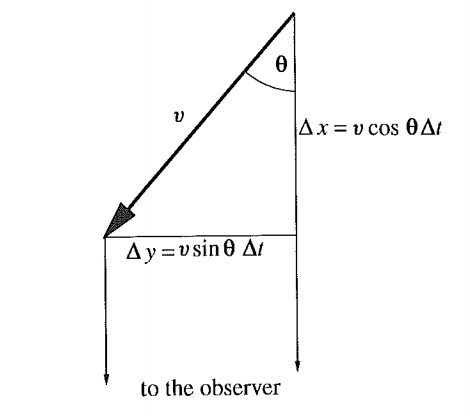
\includegraphics[width=0.5\textwidth]{jet.png} 
\caption{Jet geometry}
\label{fig_jet}
\end{figure}

Jets are collimated outflows of highly energetic plasma. Apparent superluminal motion is explained by the geometry of the jet. Imaging that you have a blob of jet material ejected at $v$ at an angle $\theta$ to the line of sight. If the transverse distance covered within the interval $\Delta t$ is $\Delta y$ \textcolor{red}{(Fig. \ref{fig_jet})}, then

$$ \frac{\Delta y}{\Delta t} = v \sin \theta $$

But, the blob is coming towards us, and the interval of time between the arrival of the two photons at our telescope is less than the interval between their emission, because of relativity:

$$ \Delta t_{\mathrm{obs}} = \Delta t (1 - \beta \cos \theta) $$

Thus, the apparent velocity is

\begin{equation}
v_\mathrm{app} = \frac{\Delta y}{\Delta t_\mathrm{obs}} = \frac{v \sin \theta}{1 - \beta \cos \theta}
\end{equation}

In radio jets, you get Lorentz factors of around 10, and in gamma ray bursts you get Lorentz factors of around 100. 

\item \textbf{Discuss the observational consequences of Doppler boosting in radio jets and in gamma-ray bursts.}

Doppler boosting: the radiation emitted by a blob of jet matter is relativistically enhanced as it approaches the observer. \textcolor{red}{\begin{equation}
\frac{I_{\nu}^\textrm{obs}}{(\nu^\textrm{obs})^3}=\frac{I_\nu^\textrm{em}}{(\nu^\textrm{em})^3}, 
\end{equation}
Because $\nu^\textrm{obs}=D\nu^\textrm{em}$, where 
\begin{equation}
D=\frac{\sqrt{1-\beta^2}}{1-\beta\cos\theta},
\end{equation}
Therefore, $I_{\nu}^\textrm{obs}(D\nu)=D^3I_{\nu}^\textrm{em}(\nu)$.
} The consequence is that the flux from the forward part of the jet is boosted by a factor of 1000 (even for a mildly relativistic jet) while the flux from the backward part of the jet is diminished by a factor of 1000. So, often, observations only show one side of the jet. However, since the radiation from jets is primarily synchrotron radiation, which usually follows a power law $I_\nu^{\mathrm{em}} \propto \nu^{-\alpha}$, the spectrum remains a power law in the observer's frame. \textcolor{red}{$I_{\nu}^\textrm{obs}=D^{3+\alpha}I_{\nu}^\textrm{em}$.}Every frequency is shifted by the same factor and the slope remains unchanged. 

\textcolor{red}{Note that for linear objects (jets), it is $I_\nu/\nu^2$ that remains constant. }

\item \textbf{What is the proposed connection between LIGO and short gamma-ray bursts?}

\textcolor{red}{The central engine is very likely to emit gravitational waves, as the energy reservoir should be much larger than the observed photon energy. Compact binary mergers are proposed to possible sources of short GRBs. The region above the poles of newly formed object is likely the place to launch fireballs because they are close to the source of energy. Neutrino annihilation can produce electron-positron pairs, and if collimated properly, can produce enough energy. }

0.4s after LIGO detected the GW event, there was a supposed gamma-ray burst detection by Fermi. However, then you'd have some missing matter. Avi Loeb's claim is that one star became two collapsing cores because it was rotating very quickly, and maybe there was a 0.4 second delay because that's the time it took the GRB to cross the star. 

\end{enumerate}

\end{document}